% Thesis introduction
% Author: Tore.
%

This chapter gives the background information needed in order to understand the topics of this thesis and the associated papers. First, in Section \ref{sec:gpgpu}, the history and the principles of general-purpose computing on graphics processing units (\nom{GPGPU}{General-purpose computing on graphics processing units}) are reviewed, followed by an introduction to medical ultrasound imaging and adaptive beamforming in Section \ref{sec:ultrasound}. Finally, the concepts of volume rendering and ultrasound field simulations are presented in Sections \ref{sec:volren} and \ref{sec:field}.

\section{General-purpose computing on graphics processing units}\label{sec:gpgpu}
Herb Sutter, a leading authority on software development, reviews the current state of the software and computer industry in a recent essay \cite{HerbSutter}. The essay bears the name "Welcome to the Jungle" and is a sequel to the essay "The Free Lunch is Over" from 2004 \cite{HerbSuttera}. The two essays spin around the fact that manufacturers of central processing units (CPUs) hit a frequency wall in the beginning of the 21st century. Until then, all mainstream computer programs where typically running in a single thread on a single CPU \textit{processing core}, and a programmer could expect the software to annually gain performance without touching the code. This was the "free-lunch" era as depicted in Fig.\,\ref{fig:jungle}. The increase in processing power came mostly from an ever-growing clock frequency. However, power consumption and heat generation were also growing at the same rate until the required cooling finally became too much in 2004.  From that point, CPU manufactures had to pursue different directions than just increasing the clock frequency. The immediate solution was to embed several cores in one CPU. This insured continuation of Moore's law, since the number of transistors per chip could continue to grow. For programmers, multi-core CPUs meant that computer programs now had to be multi-threaded in order to annually gain performance. It was a concurrency revolution, as Herb Sutter named it, and  the "free lunch" was over.

\begin{figure}
\centering
\includegraphics[width=0.8\textwidth]{img/free_lunsh.png}
\caption{Illustration of transitions between different eras in the computer industry. Currently there are three ongoing transitions; multi-core, heterogeneous-core and cloud-core. Image courtesy of Herb Sutter (herbsutter.com).}
\label{fig:jungle}
\end{figure}

Around the same time as CPU manufacturers hit the frequency wall, people had started experimenting with programmable shaders, which recently had been introduced in the field of graphics programming. The graphics processing pipeline had before this been a fixed function pipeline, where e.g. geometry and colors were fed to the graphics processing unit (GPU) in one end, and where shaded and rasterized sceneries were outputted in the other. Programmable shaders introduced the ability to replace some steps in the fixed-function pipeline with custom computations. This made it possible to utilize the GPU for other tasks than just rendering graphics \cite{Seland2007}. The rationale behind this development was that GPUs were already highly available in consumer PCs, and hidden behind its graphics interface were processing powers an order of magnitude larger than what the CPU could provide (Fig.\,\ref{fig:cpu_vs_gpu}). Actually, at the time when CPU manufacturers hit the frequency wall, the GPU had already gone multi-core, first of all driven by an ever-increasing demand for more realistic computer games. 

The original graphics pipeline involved no conditional branching, and data were typically used once \cite{Purcell2002}. Designers of GPUs could therefore skip advanced features found in most CPUs, like branch prediction and different levels of data caching. These measures reduced the silicon footprint of each core and made it possible to add multiple cores to the GPU before CPU designers where able to do the same. Today, even if more advanced caching has been added to GPUs, this is still the main reason why GPUs have higher peak performance than CPUs (Fig.\,\ref{fig:cpu_gpu} and \ref{fig:cpu_vs_gpu}). Another reason is the inherent parallel nature of the problem of rendering graphics. When geometry is shaded, projected, and rasterized, the same instruction is needed for a lot of data at the same time. This makes a special kind of instruction, known as Single Instruction Multiple Data (\nom{SIMD}{Single instruction multiple data (instruction type)}) \cite{Flynn1966}, especially suited for this problem. How SIMD instructions are utilized in modern CPUs and GPUs is discussed in Section \ref{sec:cpu_vs_gpu}.

For the first adopters of general-purpose computing on GPUs (GPGPU) it soon became evident that offloading all types of computations to the GPU was not always a good idea. In most cases it is important to balance the load equally between the CPU and GPU to get the most out of each processors. Balancing means that highly parallel and computationally intense tasks should be offloaded to the GPU while serialized and memory intensive work should stay on the CPU. This paradigm of utilizing specialized cores for solving specific problems is today known as \textit{heterogeneous computing}. The specialized core can be a GPU or e.g. a field-programmable gate array (\nom{FPGA}{Field-programmable gate array (processor)}). A recent trend is that specialized accelerator cores are embedded onto the CPU. This heterogeneous processor is often referred to as an accelerated processing unit (\nom{APU}{Accelerated processing unit}). The last three generations of CPUs from Intel have all had on-chip integrated graphics, and all of them are therefore APUs. An on-chip GPU is less powerful than a high-performance discrete GPU, but valuable time is saved by not having to send data across the PCI Express bus, which connects the different parts of a computer to the CPU. This is the reason why one of the first rules of GPGPU (with discrete GPUs) is to minimize CPU-to-GPU memory transfers. An integrated GPU can therefore provide increased performance over a discrete GPU if the problem requires a high level of CPU-GPU data synchronization.

The final transition currently taking place in the computer industry is the introduction of cloud computing, where compute power is provided as a web service and automatically scales on demand. Together, multi-cores, heterogeneous cores, and cloud cores form the "jungle" that today's software engineers have to handle (Fig.\,\ref{fig:jungle}). In this thesis we focus on heterogeneous computing with a multi-core CPU and a discrete high performance GPU. This is a cheap, high-performance system which is likely to be the specification of current and future ultrasound imaging system.

\subsection{Comparing CPU and GPU performance}\label{sec:cpu_vs_gpu}
The CPU is designed to be the main control unit of a personal computer, and is therefore good at general processing. The GPU, on the other hand, has a history of processing graphics which involves heavy vector arithmetic. Although they started out as very different processors, modern CPUs are now including more and more GPU-like features, and GPUs are adding CPU features. In this section we will see what these features are and why there is still a big difference in theoretical peak performance between a CPU and a GPU.

\begin{figure}
\centering
\includegraphics[width=0.8\textwidth]{img/CPU-GPU.pdf}
\caption{Schematic overview of CPU (Intel Haswell) and GPU (Nvidia Kepler) architectures. Note how more space is dedicated to compute cores on a GPU, and how more space is dedicated to control and caching on a CPU.}
\label{fig:cpu_gpu}
\end{figure}

In Section \ref{sec:gpgpu} a special type of instructions was mentioned, namely SIMD instructions. These are instructions which are designed to execute a single instruction across multiple data element in one clock cycle. At the end of the 20th century, Intel introduced a SIMD instruction set for their Pentium III processor called the Streaming SIMD Extensions (\nom{SSE}{Streaming SIMD extensions (instruction set)}). The first SSE instruction set had registers of 128 bit which meant that four single-precision (32 bit) floating point values could be processed per clock cycle. Updates of the SSE instruction set (SSE2, SSE3, SSE4, \nom{AVX}{Advanced vector extensions (instruction set)}, AVX2, and AVX-512) have added new instructions and longer registers. The newly introduced extensions, AVX and AVX2, add registers of 256 bit and fused multiply accumulate (\nom{FMA}{Fused multiply-accumulate (instruction)}) instructions  which means that sixteen single-precision floating point operations can be performed per clock cycle per core. A new extension, AVX-512, extends the registers to 512 bit and is found in the Intel accelerator board  Xeon Phi and might show up in the next generation of CPUs from Intel. The latest CPU architecture from Intel, the Haswell architecture, has two processing ports per core supporting FMA-AVX2 instructions, and is therefore capable of performing 32 single-precision floating point operations per clock cycle per core (Fig.\,\ref{fig:cpu_gpu}). For an eight-core\footnote{An 8-core Haswell CPU is scheduled to launch during 2014. The numbers in Fig.\,\ref{fig:cpu_vs_gpu} for the last three generations of CPUs are all based on 8-core CPUs.} CPU with a clock frequency of 3.8 GHz this sums to 
\begin{equation}
32 \times 8 \times 3.8 = 972.8\,\text{GFLOPS}.
\end{equation}
Hence, a theoretical peak performance of close to one tera single precision floating point operations per second (TFLOPS). This is the same number as visualized in Fig\,\ref{fig:cpu_vs_gpu} for the Haswell architecture (Single precision). In addition, the most powerful integrated GPU found on Haswell CPUs, the HD 5200, has 40 execution units capable of processing sixteen single-precision floating point values at 1.3 GHz. This adds
\begin{equation}
16 \times 40 \times 1.3 = 832\,\text{GFLOPS}
\end{equation}
in extra processing power to the APU.

Modern GPUs can also be interpreted as units consisting of multiple SIMD cores (Fig.\,\ref{fig:cpu_gpu}). The recent Kepler architecture from Nvidia can provide up to 15 SIMD cores\footnote{Nvidia likes to refer to the unit capable of processing one single precision floating point value as a core. In Nvidia's world, Kepler therefore has $15\times192=2880$ cores.} capable of processing 192 single-precision floating point values per clock cycle per core. These GPUs are also capable of performing FMA instructions, effectively doubling the number of theoretical FLOPS. The maximum theoretical peak single precision FLOPS for this architecture with a core frequency of 745 MHz is then found to be
\begin{equation}
15 \times 192 \times 2 \times 745 = 4291\,\text{GFLOPS}.
\end{equation} 
Each SIMD core also includes 16 special function units (\nom{SFU}{Special function unit (sin, exp, sqrt, ect.)}) which add close to 1 TFLOPS in additional computational power. This adds up to a total of 5 TFLOPS as shown in Fig.\,\ref{fig:cpu_vs_gpu} for the GeForce GTX 780 TI GPU. From Fig.\,\ref{fig:cpu_gpu} we see how the high number of SIMD cores found on GPUs and their larger width, compared with the SIMD cores on CPUs, results in five times the computational performance of a high-end CPU (without the integrated GPU). 

Note that the derived numbers are strictly theoretical and that the actual throughput is highly algorithm dependent. Nevertheless, in theory, the computational power provided by modern GPUs is five times higher than that provided by CPUs. A claimed speed-up of several orders of magnitude is therefore typically a result of comparing a non-optimized CPU implementation with an optimized GPU implementation or by comparing uneven hardware \cite{Lee2010, Kothapalli2013}. However, in the next section we will see why it is often easier to obtain an optimized implementation for the GPU than for the CPU.

In this section we have focused on CPUs from Intel and GPUs from Nvidia, however, CPUs and GPUs from AMD have similar specifications and differences in theoretical peak performance. 

\begin{figure}[t!]
\centering
\includegraphics[width=\textwidth]{img/cpu_vs_gpu.pdf}
\caption{Development in theoretical peak throughput, single precision (SP) and double precision (DP), the last decade for Intel CPUs and Nvidia GPUs.}
\label{fig:cpu_vs_gpu}
\end{figure}

\subsection{Programming a GPU}
Early GPGPU programming required expert knowledge of computer graphics and the graphics pipeline. When GPGPU gained a broader interest and the GPU started to be used to compute problems that did not involve graphics, it quickly became evident that new programing languages where needed.  One of the first GPGPU oriented languages was the Brook language by Buck \textit{et al.} \cite{Buck2004}. Buck later joined Nvidia where he led the work on \nom{CUDA}{Compute unified device architecture (GPGPU framework)}, a GPGPU language and framework by Nvidia for Nvidia GPUs only. The first version of CUDA was released in 2007. The following year, Apple launched a GPGPU framework known as \nom{OpenCL}{Open Compute Language (GPGPU framework)}, a standard which is maintained by the Khronos Group. These two frameworks are still today the main programming frameworks for GPGPU. While CUDA only runs on Nvidia GPUs, OpenCL can now run on GPUs from both Nvidia and AMD, CPUs from both Intel and AMD, FPGAs from Altera, and mobile processors from \nom{ARM}{Designer of mobile chip architectures}.

\begin{figure}[t!]
\centering
\subfloat[Kernel]{
	\includegraphics[width=0.5\textwidth]{img/kernel.pdf}\label{fig:gpu_kernel}
}
\subfloat[Threads, blocks and grid]{
	\includegraphics[width=0.4\textwidth]{img/cuda_threads.png}\label{fig:gpu_grid}
}
\caption{The figure depicts how GPU threads are grouped into blocks and arranged in a grid. One thread runs a copy of a kernel function. In this example the kernel function performs an in-place element-wise matrix square.}
\label{fig:gpu_grid_kernel}
\end{figure}

Both CUDA and OpenCL are centered around a kernel function which is executed by a large group of threads. The kernel function, for both CUDA and OpenCL, has a C-like syntax with some additional specifiers. An example of a CUDA kernel is depicted in Fig.\,\ref{fig:gpu_kernel}. The \texttt{\_\_global\_\_} specifier tells the CUDA compiler that this function is a kernel function, and in CUDA this kernel function is launched by using a CUDA-specific syntax:
\begin{align*}
\texttt{square<<<grid, block>>>(a, N)},
\end{align*}
where \texttt{grid} and \texttt{block} are 3-component vectors specifying grid and block size in "xyz" as depicted in Fig.\,\ref{fig:gpu_grid}, \texttt{a} is a pointer to a memory buffer located on the GPU, and \texttt{N}$*$\texttt{N} is the size of the buffer \texttt{a}. 

When the kernel is launched, a copy of it is scheduled for each thread in each block, and each kernel instance gets as input its location in the grid (\texttt{blockIdx} and \texttt{threadIdx}) together with the grid size (\texttt{gridDim} and \texttt{blockDim}). This information is then typically used to calculate which values to gather from the global memory, in this case an element of \texttt{a}. %Behind the scene, thread blocks are divided into smaller sets of threads called a warp (or wavefront in OpenCL). 
When a kernel is executed, multiple arbitrary thread blocks are scheduled to each SIMD core where they stay until all instructions in the kernel are finished for all threads in all the blocks. This step is then repeated until all blocks have been processed. Thus,  in order to formulate a given problem as a kernel function, it must be possible for the GPU to schedule the resulting thread blocks in any order. As an example, the global memory input to each thread can therefore not depend on the output from other blocks.

As we see, a thread has a different conceptual meaning on a GPU than on a CPU.  While a CPU is said to execute threads which can perform SIMD instructions, a thread on a GPU can be interpreted as a unit capable of processing one data element in the SIMD instruction. The GPU is because of this sometimes referred to as a single instruction multiple threads (\nom{SIMT}{Single instruction multiple threads}) processor instead of a SIMD processor. This also explain why GPU threads are said to be light-weighted. Such a conceptual difference means that there is an inherent focus on breaking algorithms down into SIMD instructions when programing for the GPU. This often leads to a highly optimized parallel implementation on the GPU and not on the CPU. Manually typed SIMT, or SIMD, instructions is the only way of programming the GPU, while a single thread with automatic vectorization of for-loops is the standard way of programming the CPU. 

It is important to understand that not all algorithms will benefit from wider SIMD registers. As the width increase, the only algorithms that will benefit are those which can be divided into a sufficiently large number of independent calculations. Also, to achieve peak performance, the implementation must perform one FMA operation on each core per clock cycle, and it must be possible for the GPU to hide all memory latency by scheduling threads which are not stalled by a memory fetch. All of this is something which is impossible to achieve in practical applications, and therefore one will always end up with a throughput which is a fraction of the peak throughput.

The code in Fig.\,\ref{fig:gpu_grid} is an incomplete and minimal example of a GPU program. A full example will involve several lines of C++ code transferring data to and from the GPU, and the kernel could include manual administration of the L1 cache (shared memory), and intra-block thread barriers. This is part of the reasons why writing a high performance GPU kernel is often found to be a complex and time consuming task. Therefore, we will probably see a lot of work aimed at reducing this overhead in the future.  A recent development is the introduction of C++ AMP which enables developers to write accelerated code (e.g. by a GPU) in plain C++. Hopefully, in near future, programming the GPU will be a job for compilers, and direct fiddling with GPU kernels should only be needed if maximum throughput is absolutely needed. This is similar to how SIMD instructions are handled in CPU-code today. Most of the time developers will rely on the CPU compilers to analyze the code and auto-apply SIMD instruction whenever it is possible. However, when maximum throughput is needed, developers with deep knowledge of the algorithm are often able to make faster code by manually writing SIMD instruction. The relevance of auto-applied GPU instructions will also increase due to the recent embedding of GPUs on the same chip as the CPU. Soon, GPU programming will probably be a matter of coding a heterogeneous collection of cores where operations are automatically offloaded to the right core (e.g. a GPU) by the compiler.

\section {Medical ultrasound imaging}\label{sec:ultrasound}
Medical ultrasound imaging is considered to be a low-risk tool for non-invasive investigation of the human body. Neither gamma rays nor high intensity magnetic fields are involved, just sound pressure below well-controlled limits. It is also far less costly than other medical imaging modalities and offers real-time imaging. Ultrasound imaging is well known for its use in fetal imaging during pregnancy, however, in this thesis we will focus on a different modality, namely cardiac ultrasound imaging. An illustration of the human heart is therefore included in Fig.\,\ref{fig:human_heart}. Throughout the thesis we will refer to some of the parts shown in Fig.\,\ref{fig:human_heart}. Especially note the four chambers of the heart, the left and right atrium, and the left and right ventricle. The tissue separating the left and right ventricle is known as the inter-ventricular septum. The left side is responsible of pumping blood out to the whole body through the aortic valve. It is therefore the strongest and hardest working part of the heart. When blood flows out of the aorta, it is important that the mitral valve, which separates the left atrium from the left ventricle, is closed and does not leak. The left side, and especially the left ventricle and the mitral valve, therefore receives the most attention during cardiac ultrasound examinations. When visualizing 3D ultrasound images in \textbf{Paper IV} we will have a strong focus on visibility of cardiac tissue, thus note for later that the endocardium refers to the innermost layer of the cardiac muscle.

\begin{figure}
\centering
\subfloat[]{
	\includegraphics[width=0.47\textwidth]{img/Diagram_of_the_human_heart.png}\label{fig:human_heart}
}
\subfloat[]{
	\includegraphics[width=0.47\textwidth]{img/ultrasound_grid.pdf}\label{fig:us_grid}
}
\caption{a) Overview of the human heart. Illustration from wikipedia.org. b) Illustration of probe geometry and layout for phased array imaging.}
\end{figure}

%Ultrasound imaging encompasses technology which generates images based on sound whose frequencies we can not hear. For medical ultrasound imaging frequencies between 2 MHz and 10 MHz are typically used. The choice of frequency depends on the depth of the body layers we want to image, because human tissue exhibits frequency dependent attenuation. This is why a frequency around 3 MHz is used for fetal and cardiac imaging and a frequency around 7 MHz is used for more shallow imaging (e.g. vascular imaging). 

To generate the ultrasonic frequencies used for imaging, a piezoelectric ceramic is used. A piezoelectric material has a special property where mechanical vibrations are generated when voltage is applied and \textit{vice versa}. It can therefore be used to both send and receive ultrasound signals, like a combined microphone and speaker. A set of piezoelectric elements organized in an array is referred to as an ultrasound \textit{probe}, and special probes are typically designed for different medical imaging modalities. An example of a probe for medical ultrasound imaging is shown in Fig.\,\ref{fig:us_grid}. %For cardiac ultrasound imaging the probe must not only be designed for a certain frequency range, its footprint also needs to be smaller than the intercostal window in order to avoid shadowing by ribs. 

If the width of a piezoelectric element is less than the wavelength of the transmitted signal the element is said to be \textit{omnidirectional}, hence, energy will be distributed or sensed equally in all directions. When multiple omnidirectional elements are arranged in an array, the transmitted pulse will get shaped into a beam\footnote{A beam refers to the accumulated magnitude across time of a pulse traveling in space.} of ultrasound by diffraction as the width (the \textit{aperture}) of the array grows. The angular width of this beam, and also the angular resolution in radians of the array, is approximately given by \cite{AngelUltrasound}:
\begin{align}\label{eq:res}
\delta\theta_a = \frac{\lambda}{D} = \frac{c}{fD},
\end{align}
\nomi{$\delta\theta_a$}{Angular resolution of an aperture}where \nom{$\lambda$}{Wavelength} and \nom{$f$}{Frequency} are the ultrasound wavelength and frequency respectively, $c$ is the speed of sound in human tissue, and \nom{$D$}{Aperture size} is the aperture width. With an average speed of sound in human tissue of $1540\frac{\text{m}}{\text{s}}$, the angular resolution or opening angle of a 2 cm cardiac probe operating at 3 MHz is around 1.5\degree. The axial resolution is inversely proportional to the pulse length, and is typically better than the lateral resolution. An overall view of the cardiac ultrasound imaging geometry is depicted in Fig.\,\ref{fig:us_grid}. A line in the depicted ultrasound image is generated by firing an ultrasound pulse or beam into the body and sample the received echo. We will refer to this amplitude trace as an \textit{image line}. 

\subsection{Beamforming}
If time delays are applied to the signal emitted by the elements it is possible to steer and focus the ultrasound beam in space (Fig.\,\ref{fig:das_background}). This technique is known as \textit{beamforming}, and for ultrasound imaging it is applied both when transmitting and receiving ultrasound pulses. A cardiac probe is a phased probe, which means that the image is constructed from image lines which are gradually steered from $-\theta/2$ to $\theta/2$ radians. As depicted in Fig.\,\ref{fig:us_grid}, this results in an imaging sector which is $\theta$ radians wide. This is known as a 2D B-mode image (B for brightness). If image lines are acquired for multiple B-mode images that are tilted in the $yz$-plane we get what is known as a volumetric B-mode or a 3D ultrasound image. A probe for 3D imaging has several thousand elements arranged as a matrix in order to facilitate steering in both the $xz$ and $yz$ planes. In this thesis we will focus on 2D imaging when the topic is adaptive beamforming, and 3D imaging when the topic is adaptive visualization.

\begin{figure}
\centering
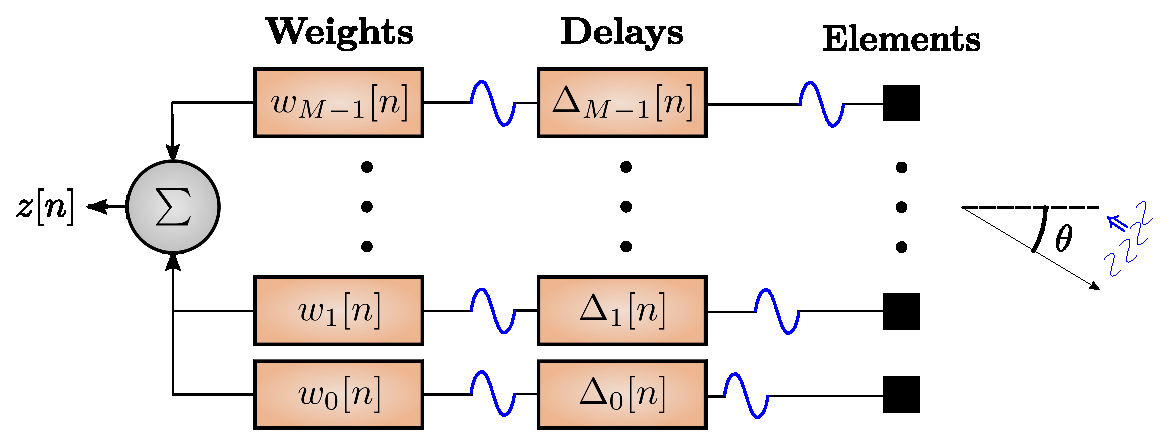
\includegraphics[width=0.8\textwidth]{img/beamforming_das.eps}
\caption{Delay-and-sum array beamforming.}
\label{fig:das_background}
\end{figure}

The standard form of beamforming used in ultrasound imaging is known as \textit{delay-and-sum} (DAS): 
\begin{align}\label{eq:das_background}
z[n] = \sum_{m = 0}^{M-1}w_m^*x_m[n - \Delta_m[n]] = \vec{w}^H\vec{x}[n].
\end{align}
Here, \nom{$M$}{Number of array elements} is the number of elements in the array, $x_m$ is the per-element data, \nom{$\Delta_m$}{Per-element focusing and steering delays} is the per-element focusing and steering delay, \nom{$\vec{w}$}{Array weight vector (apodization)} is the array \textit{weight vector} or \textit{apodization}, $\vec{x}$ is a pre-delayed vector of element data, and $z[n]$ is the output image line in the direction given by $\{\Delta_m[n]\}$.  From now on we will omit the dependency on $\{\Delta_m[n]\}$ and $x_m$ will refer to delayed element data. A schematic overview of delay-and-sum array beamforming is depicted in Fig.\,\ref{fig:das_background}. If $p_o$ is the phase center of our array and $p$ is the point to which we want to steer and focus the ultrasound beam, we have to use the following delays:
\begin{align}
\Delta_m[n] =\frac{|p_o+p| - |p_m+p|}{c},
\end{align}
where \nom{$c$}{Speed of sound} is the speed of sound in human tissue, and $p_m$ is the position of the m'th element. When transmitting the pipeline depicted in Fig.\,\ref{fig:das_background}, without the sum operator, is reversed and the negated set of delays has to be used. Also note that on transmit we have to decide where to steer and focus prior to transmitting a pulse. Transmit delays therefore do not vary within an image line.

\subsection{Sampling and processing complexity}
When generating a B-mode image, we have to insure that the spatial and temporal sampling are sufficient. We have already seen that the lateral resolution of an ultrasound probe is given by (\ref{eq:res}).  Hergum \textit{et al.} \cite{Hergum2009} have further shown that the lateral frequency support for a system that both emits and receives energy is governed by the sum of the transmit ($D_{tx}$\nomi{tx}{Transmit}) and receive ($D_{rx}$\nomi{rx}{Receive}) aperture. The lateral resolution of what is known as an active imaging system is found to be
\begin{align}
\delta\theta = \frac{\lambda}{D_{tx} + D_{rx}}.
\end{align}
\nomi{$\delta\theta$}{Angular resolution of a two-way imaging system}\nomi{$D_{tx}$}{Aperture size on transmit}\nomi{$D_{rx}$}{Aperture size on receive}Then, in order to properly sample an imaging sector of $\theta$ radians we have to acquire 
\begin{align}
N_\theta = \frac{\theta}{\delta\theta}
\end{align}
\nomi{$N_\theta$}{Number of lines required for proper sampling of an imaging sector}image lines distributed across the imaging sector. If \nom{$r$}{Imaging range.} is the maximum range in our image, as shown in Fig.\,\ref{fig:us_grid}, we can acquire
\begin{align}
f_{\text{FPS}} = \frac{c}{2rN_\theta}
\end{align} 
images or frames per second (\nom{FPS}{Frames per second}). With our 2 cm cardiac probe we get a frame rate of around $55$ FPS when imaging a 70\degree{} sector with $r=15$ cm.

The required axial sampling is dictated by the transmit frequency and the frequency bandwidth of the probe. From Fourier theory we know that a short pulse consists of many frequency components. A short ultrasound pulse, which would yield a high axial resolution, requires therefore a large frequency bandwidth. Medical ultrasound systems typically has a bandwidth between 33 \% and 100 \% of the pulse frequency. This corresponds to transmitting a pulse which is between 1 and 3 oscillations when entering tissue. In the analog-to-digital converter of an ultrasound imaging system a high sampling frequency is typically used (e.g. 40 MHz). However, the ultrasound signal is band limited, and the data rate can therefore be reduced in a process known as \textit{in-phase quadrature (\nom{IQ}{In-phase quadrature (ultrasound data format).}) demodulation}. In this process the axial sampling rate is reduced to the bandwidth of the imaging system in the following three steps: demodulation with a complex exponential, low-pass filtering, and decimation. The number of samples in one image line is after this process given by:
\begin{align}
N = \frac{2r}{c}B_wf_c,
\end{align}
\nomi{$N$}{Number of samples in range (or time)}where $f_c$ is the center frequency of the transmitted pulse, and where \nom{$B_w$}{Relative bandwidth} is the relative bandwidth in percent of \nom{$f_c$}{Center frequency of ultrasound pulse}. Note that after this process the ultrasound data will be complex values. The total number of samples in an B-mode image from a phased array is then 
\begin{align}
N_{\text{B-mode}} = N_\theta N.
\end{align}
If our cardiac probe, which is used to image a $70$\degree{} sector, has a relative bandwidth of $80$ \% we have to process almost $50000$ complex data vectors of length $M$ every $1/55$ second. The formula for the number of FLOPS required for real-time DAS beamforming of cardiac ultrasound is then roughly given as:
\begin{align}
\text{FLOPS}_{\text{DAS}} = MN_{\text{B-mode}}f_{\text{FPS}} = MB_wf_c.
\end{align}
If our cardiac probe has $M=128$ elements, DAS beamforming requires a processing throughput of around $300$ MFLOPS. This is far below the peak processing throughput of modern GPUs and CPUs. The main challange with DAS beamforming is the amount of data that has to be moved. In our example, for a sample size of four bytes, around 1.2 GB has to be moved to the GPU every second. This is however less than the maximum bandwidth of PCI Express 2.0 (8 GB/s), even after the relative bandwidth, transmit frequency and number of array elements are increased with a total factor of 5. Newer versions of PCI Express, which supports even higher transfer rates, have also recently been introduced.

%Time v.s. phase delays. It is well described in the paper using phase delays.

\subsection{GPUs in medical ultrasound imaging}
Ultrasound scanners generate an incredible amount of data. A modern system capable of 3D imaging will generate several tera-bytes of data inside the probe handle during a clinical scan. Fortunately the data rate is reduced to the level of 2D imaging before the data reaches the scanner. The data rate of a 2D scan is "only" in order of giga-bytes per second. To handle this amount of data, ultrasound imaging systems have, for the last twenty years, relied heavily on application-specific integrated circuits (\nom{ASIC}{Application-specific integrated circuit}) for all steps in the processing pipeline \cite{Thomenius}. However, as the computational power of generic processors have increased, the expensive ASICs have gradually been replaced by software \cite{Guracar2013}. One of  the last remaining ASICs in ultrasound scanners is used for beamforming \cite{Thomenius}. As seen from (\ref{eq:das_background}), beamforming involves a reduction of the data rate with a factor equal to the number of elements in the ultrasound probe. The input data rate is therefore very high. Nevertheless, real-time beamforming has recently been achieved on a GPU \cite{Song2012}, and a French company (SuperSonic Imagine) are utilizing GPUs in their plane wave beamforming algorithm \cite{Tanter2014}. This is the same technique as reported implemented on a GPU by Yiu \textit{et al.} \cite{Yiu2011}. We can therefore conclude that beamforming is finally moving into software too. The largest players in the medical ultrasound business, General Electric and Philips, are also well aware of where the trend is going \cite{Thomenius2012} \cite{Metz2011}. 

Software beamforming opens up for cost-efficient and rapid prototyping of advanced processing of ultrasound data. One example is Capon beamforming which is explored in this thesis (\textbf{Paper\,I} and \textbf{II}) and introduced in the next section. The increased computational power introduced by GPUs makes it also possible to include more advanced 3D visualization as presented in \cite{solteszova2010multidirectional}, \textbf{Paper\,IV}, and \textbf{IX}.

\subsection{Adaptive beamforming}\label{sec:adaptbf}
Adaptive beamforming has several meanings in the medical ultrasound imaging literature. It can for instance refer to aberration correction \cite{cole1996method} which is the task of applying time delays to compensate for pulse distortion introduced by fatty layers in the human body. However, in this thesis adaptive beamforming will refer to data-dependent weighting derived from a given optimization criterion. The optimization criterion that we focus on in this thesis is the minimum variance distortionless response criterion, which is also known as Capon's method \cite{Capon1969}. A beamformer that uses weights derived with Capon's method will in this thesis mainly be referred to as the \textit{Capon beamformer} \cite{Vignon2008}. However, it is also known as the minimum variance  (\nom{MV}{Minimum variance beamformer (Synonym for Capon)}) beamformer \cite{Synnevag2007}, the minimum variance distortionless response beamformer (\nom{MVDR}{Minimum variance distortionless response beamformer (Synonym for Capon)}) [\textbf{Paper I}], or the constrained adaptive beamformer \cite{Mann2002}.

\begin{figure}[t!]
\subfloat[Uniform weights]{
	\includegraphics[width=0.47\textwidth]{img/scenario_das_resp2.png}\label{fig:das_weights}
}
\subfloat[Capon weights]{
	\includegraphics[width=0.47\textwidth]{img/scenario_mv_resp2.png}\label{fig:capon_weights}
}
\caption{Examples of array beampatterns where the array weights are either uniform (a) or derived using Capon's method (b). An interfering source is located at 20\degree. Notice the reduced sidelobe level for the Capon beampattern in the direction of the interfering source. Image courtesy of Jo Inge Buskenes.}
\label{fig:weights}
\end{figure}

The Capon beamformer produces a weight vector, as introduced in (\ref{eq:das_background}), based on the impinging signal and a constrained optimization problem. The problem is as follows \cite{Capon1969}:
\begin{align}
&\min_{\vec{w}} E\{|z[n]|^2\} \approx \min_{\vec{w}} \vec{w}^H \mat{\hat{R}} \vec{w} \label{eq:capon_optimization_criteria_background} \\
&\text{subject to } \vec{w}^H\vec{a} = 1,\notag
\end{align}
where \nom{$\mat{\hat{R}}$}{Sample covariance matrix (with regularization)} is a sample covariance matrix, and \nom{$(.)^H$}{Complex conjugate transpose} is the complex conjugate transpose. Hence, the resulting weight vector minimizes the output power (the criterion) while maintaining unit gain in the steering direction $\vec{a}$ (distortionless response). The benefit of Capon beamforming is clearly seen from Fig\,\ref{fig:weights}, which presents a sensitivity map (an \textit{array beampattern}) for DAS beamforming with uniform weights and the Capon beamformer. In this simulated case, an interfering source is located at 20\degree{}, which for the DAS beamformer with uniform weights (\ref{fig:das_weights}) will leak into the beamformer output with its power attenuated by around $13$ dB. Since the Capon weights are data-dependent, the method "knows" where the interfering source is located and is able to position a zero in its direction (Fig.\,\ref{fig:capon_weights}). Hence, the interfering source will be highly attenuated independent of the direction from which it arrives. Another interesting case is when the interfering source is located within the mainlobe of the array beampattern. In theory a signal will be regarded by the Capon beamformer as an interfering source as long as the signal propagation vector does not match the steering vector ($\vec{a}$) exactly. Positioning of a zero in the direction of an interferer within the mainlobe will lead to a shifted and scaled mainlobe if this is what is needed in order to achieve minimum output power. Adaptive positioning of zeros and mainlobe shifting are the source to the super-resolution capabilities of the Capon beamformer \cite{Synnevag2007}, and the positive implications of this effect \cite{Synnevag2009} is the main reason why this beamformer has been highly studied in the field of medical ultrasound imaging over the last decade.

To "know" the direction of interfering sources the Capon beamformer has to estimate the statistics of the impinging wave field. This is done by estimating a sample covariance matrix, which for an active broadband system can be done in the following way \cite{Synnevag2009}:
\begin{align}
\mat{\breve{R}}[n] &= \frac{1}{N_LN_K}\sum_{n'=n-K}^{n+K} \sum_{l=0}^{N_L-1} \vec{x}_l[n']\vec{x}_l[n']^H\\
\vec{x}_l[n'] &= [x_l[n'], \dotso, x_{l+L}[n']]
\end{align}
where\nomi{$K$}{Temporal averaging parameter (Capon)} $N_K = 2K + 1$ \nomi{$N_K$}{Number of samples used for temporal averaging (Capon)} is the number of samples used for temporal smoothing,\nomi{$L$}{Subarray length (Capon)} $\vec{x}_l$ is a subarray of length $L$, and $N_L = M-L+1$\nomi{$N_L$}{Number of subarrays used for spatial averaging (Capon)} is the number of subarrays used for spatial averaging.  Temporal averaging is used to obtain DAS-like speckle statistics in combination with large subarrays \cite{Synnevag2007a}, and subarray averaging is applied to reduce signal cancellation caused by coherent signals \cite{Reddy1987}. The number of temporal samples is selected relative to the pulse length. To ensure robustness against model errors and numerical stability the matrix is further loaded with a diagonal factor, 
\begin{align}
\epsilon &= d\times\text{trace}\{\mat{\breve{R}}\}/L\\
\mat{\hat{R}} &= \mat{\breve{R}} + \epsilon\mat{I}.
\end{align} 
Hence, a white noise component proportional to the in-coherent signal power is added to the estimate \cite{Featherstone1997b}.

The solution to the constrained minimization problem in (\ref{eq:capon_optimization_criteria_background}) is, by the method of Lagrange multipliers \cite{VanTrees2003}, found to be
\begin{align}\label{eq:capon_weights}
\vec{w}[n] = \frac{\mat{\hat{R}}[n]^{-1}\vec{a}}{\vec{a}^H\mat{\hat{R}}[n]^{-1}\vec{a}} \in \mathbb{C}^L.
\end{align}
Since $\vec{w}$ is time (or range) dependent, a matrix has to be constructed and inverted for each data vector $\vec{x}[n]$ received by the system. This is indeed computationally demanding, something which becomes clear when each step of the beamformer is examined closer. It is then found that constructing the covariance matrix has a computational complexity of $O(L^2N_LN_K)$\nomi{O(.)}{Big O notation (algorithm complexity)}, inverting it has a computational complexity of $O(L^3)$, and the final normalization and calculation of $\vec{w}$ is $O(L)$. For $L=M/2$, a subarray size often used in the literature, the first two steps both have a complexity of $O(L^3)$. These steps should therefore receive the same amount of attention when a real-time implementation of Capon beamforming is attempted.

A rough estimate of the number of FLOPS required by a Capon beamformer for real-time cardiac ultrasound imaging is then given by:
\begin{align}
\text{FLOPS}_{\text{Capon}} = L^3B_wf_c.
\end{align}
Which for our example, with $L=M/2=64$, sums up to a required throughput of more than $1/2$ TFLOPS. Even though this is just 10\% of the peak throughput of modern GPUs, remember that the latter are only theoretical numbers, and that the actual throughput is highly algorithm dependent. The required throughput for Capon beamforming might therefore still be hard to achieve in practice \cite[\textbf{Paper II}]{So2011}. As for DAS beamforming, this number also scales with higher relative bandwidth, pulse frequency, and more array elements since the subarray size is typically proportional to the number of array elements. 

In the medical ultrasound imaging literature we find few attempts of implementing a Capon beamformer for real-time imaging. In addition to the papers in this thesis only Chen \textit{et al.} \cite{Chen2011, Chen, Chen2011a} are known to have explored GPU and FPGA implementations of the Capon beamformer for medical ultrasound imaging. The differences between our work and Chen \textit{et al.} is discussed in \textbf{Papers I}, \textbf{II}, and \textbf{VI}.

To reduce the processing requirement of the Capon beamformer for medical ultrasound imaging, several simplified version have been proposed in the literature \cite{Asl2012, Kim}. Among the most interesting proposals we find the low complexity adaptive (LCA) beamformer by Synnev\aa{}g \textit{et al.} \cite{Synnevag2011} and the beamspace (BS) Capon beamformer by Nilsen and Hafizovic \cite{Nilsen2009}. In medical ultrasound imaging beamspace typically refers to the polar grid that cardiac ultrasound data are located in prior to scan conversion. In combination with the Capon beamformer, beamspace refers to the wavenumber-space representation of the recorded signals, i.e., the spatial Fourier transform of the element data: 
\begin{align}
\vec{x}_{\text{BS},l} &= \mat{B}[x_l[n],\,\dotso,\,x_{l+L}[n]]^T\\
[\mat{B}]_{p,q} &= \frac{1}{\sqrt{L}}e^{-j 2 \pi p q / L}.
\end{align}
The idea behind BS-Capon beamforming is that spatial beams with little information can be removed from $\mat{\hat{R}}$ by removing rows in $B$. When investigating the complexity of the BS-Capon beamformer [\textbf{Paper II}] we find that it is dominated by the transformation of data into beamspace, $O(N_LLN_b)$, where \nom{$N_b$}{Number of selected beams in beamspace (BS-Capon)} is the number of selected beams. 

The number of FLOPS required for BS-Capon beamforming of real-time cardiac ultrasound is then found to be around:
\begin{align}
\text{FLOPS}_{\text{BS-Capon}} = N_LLN_bB_wf_c
\end{align}
For our example, BS-Capon beamforming with $L=M/2=64$ and $N_b=3$ will require a throughput of around $30$ GFLOPS. This is a level of processing which both modern CPUs and GPUs should be able to handle. A GPU implementation of the BS-Capon beamformer for real-time cardiac ultrasound imaging is presented in \textbf{Paper II}. The rationale behind using the GPU is that in the heterogeneous computing paradigm a highly parallel task like the Capon and BS-Capon beamformer should be offloaded to the processor made for parallel processing. The CPU is then left to do managing and all the tasks it traditionally performs. It should also be possible to achieve higher processing throughput on a GPU than on a CPU for this kind of problem.

\subsection{Narrowband or broadband Capon beamforming}
Both the LCA and BS-Capon beamformers are based upon a detailed investigation of how Capon beamfoming behaves when applied to medical ultrasound images. For the LCA beamformer, the windows selected by the Capon beamformer were investigated and a special set of predefined windows were defined. If one looks closer at the windows selected for the LCA beamformer we see that half the set performs micro-steering of the mainlobe and the other half provides different mainlobe widths. The results from applying the LCA beamformer show that the main benefit of applying Capon beamforming to medical ultrasound imaging is micro-steering of the mainlobe, and not attenuation of far off-axis backscatter.

The Capon beamformer is derived for narrowband applications and has traditionally been applied to medical ultrasound imaging "as is". Medical ultrasound imaging is, however, a broadband imaging modality and one could think that a broadband Capon beamformer would therefore be needed \cite{Holfort2009}. The investigation performed in \cite{Nilsen2009} showed, that with pre-delayed data, energy will be centered on-axis and as little as three near-axis beams is therefore adequate in order to achieve similar performance for BS-Capon and Capon beamforming. The two-way beam will be wider for unfocused (plane wave) transmit beams \cite{Holfort2009, Austeng2011}, but steering and focusing on receive will still make the main amount of energy arrive on axis. As shown in \textbf{Paper III} it is also possible to micro-steer with phase delays (narrowband) instead of time delays (broadband) without introducing large errors. Since Capon beamforming mainly performs main-lobe shifts smaller than the beam width, the difference between a broadband and narrowband Capon beamformer will be minimal \cite{Diamantis2014}. Broadband Capon beamforming is also significantly more computationally demanding than narrowband Capon beamforming.

%A final important point when working with Capon beamforming is how we present our results with respect to normalization. Since the Capon beamforming highly attenuate signals within the mainlobe  we can get a false impression of improvements in contrast if we normalize  \cite[Fig.\,6]{Synnevag2007}
%\todo{Need figures here...}

%Examples of other adaptive apodization methods found in the literature on medical ultrasound imaging includes the APES beamformer, the MUSIC method, and the eigenvalue method. \todo{Need references}.		
																						
%\subsection{Shift invariance}

%One sentence about speckle tracking.

\section{Volume rendering}\label{sec:volren}
\begin{figure}[t!]
\centering
\subfloat[Ray-casting]{
	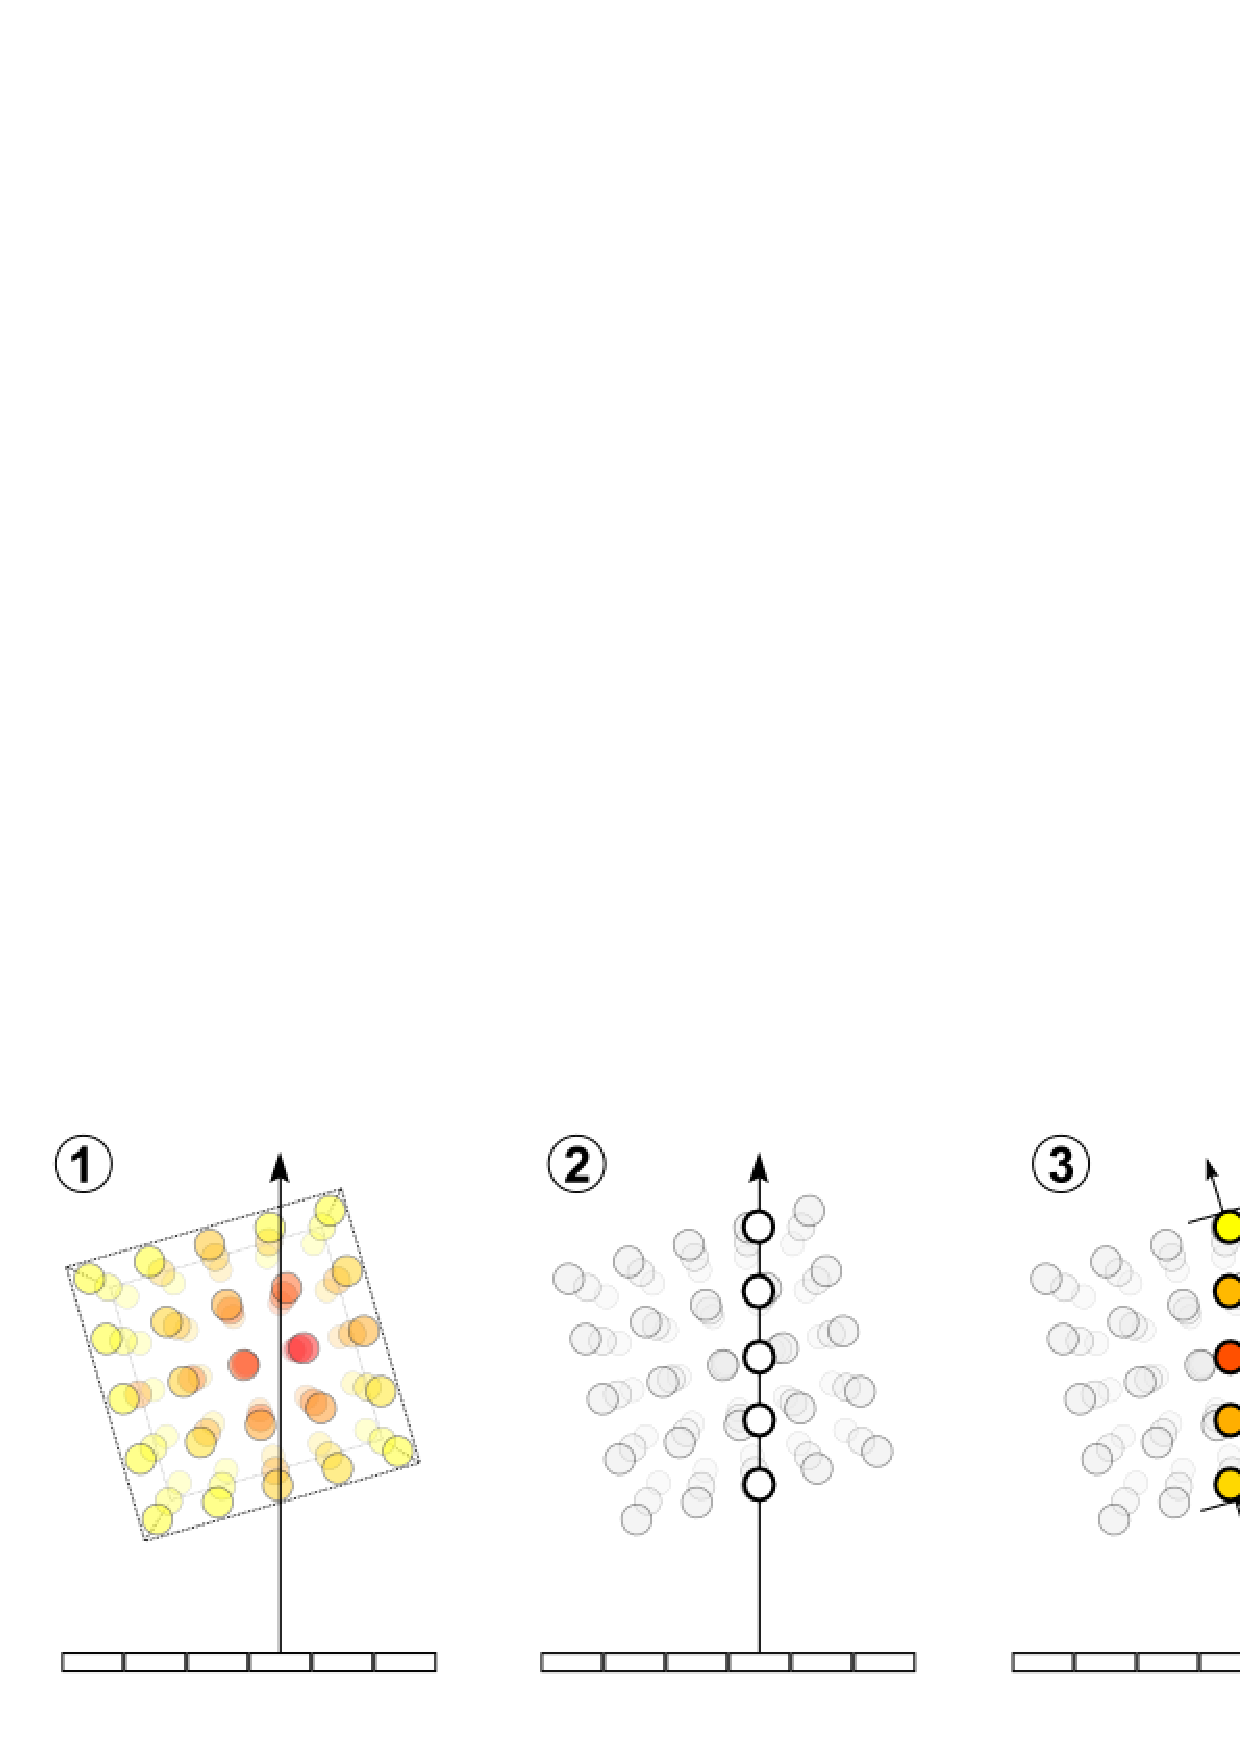
\includegraphics[width=0.4\textwidth]{img/Volumeraycasting.png}\label{fig:vr_rc}
}
\subfloat[Opacity transfer function]{
	\includegraphics[width=0.5\textwidth]{img/otf.png}\label{fig:vr_otf}
}
\caption{The principle behind volume ray casting. a) A ray is casted out from every pixel in the output image. Along the ray, samples are gathered from the volume. The samples are assigned a color and an opacity before they are combined into one pixel value. b) The opacity transfer function used to determine how opaque a sample should be.}
\label{fig:vr}
\end{figure}
A 3D ultrasound dataset is a cloud of scalar values that somehow needs to be presented to the user. One approach used for cardiac ultrasound  is to extract slices corresponding to different long-axis and short-axis views of the cardiac chambers. Another way is to project the whole volume into a two-dimensional image. The latter technique is known as volume rendering, and it presents to the user the three dimensional structure of the heart in one two-dimensional image. Many different methods for volume rendering exist \cite{brodlie2001}, but in this thesis we will focus on ray casting \cite{Levoy1988}. 

The principle behind ray casting is depicted in Fig.\,\ref{fig:vr}. The projection of volumetric data is performed by casting a ray out from every pixel in the output image (Fig.\,\ref{fig:vr_rc}). Along each ray, samples are gathered from the volume and assigned color and opacity. For ultrasound visualization, the color intensity is dictated by the ultrasound backscatter intensity, and the actual color is often encoded with depth information in order to improve depth perception. An example of a volume rendering of cardiac ultrasound data is presented in \textbf{Paper IV}. The opacity, however, is governed by a user-controlled \textit{opacity transfer function} (\nom{OTF}{Opacity transfer function (volume rendering)}) as shown in Fig.\,\ref{fig:vr_otf}. For ultrasound visualization a monotonically increasing function is typically used, which means that below a certain threshold all samples will be rendered transparent (opacity = 0). We will refer to this as the \textit{opacity threshold}, and for the example in Fig.\,\ref{fig:vr_otf} this threshold is 25.

The iterative composition scheme for front-to-back ray casting of one ray, from $s_0$ to $s_{N_s-1}$ where $s$ is the sample position and $N_s$ is the number of samples along the ray, is \cite{rtvg2006}
\begin{align}
I(s_0, s_{i+1}) &= I(s_0, s_{i}) + (1 - \alpha_{\text{acc},i}) c_{i+1}\\
\alpha_{\text{acc},i+1} &= \alpha_{\text{acc},i} + (1 - \alpha_{\text{acc},i}) \alpha(c_i+1).
\label{eq:fronToBack}
\end{align}
Here, $\alpha(v)$ is the opacity transfer function, $c_{k}$ is the color intensity of sample $s_{k}$, $\alpha_{\text{acc}}$ is the accumulated opacity, and $I(s_0, s_{N_s-1})$ is the intensity value of all the projected samples combined. If $\alpha(v)$ is close to one for one or two consecutive samples, $\alpha_{\text{acc}}$ will quickly approach a value of one. An $\alpha_{acc,k}$-value close to one means that the contribution from $c_{k+1}, \cdots, c_{N_s-1}$ to the final value, $I(s_0, s_{N_s-1})$, will be minimal. Hence, the iteration can stop at $i=k$ without loosing visible samples. This optimization technique is known as \textit{early-ray-termination}, and will significantly speed up the rendering algorithm if an opaque material is rendered.

For visualization of cardiac ultrasound we want $\alpha_{\text{acc}}$ to be close to one only when a tissue interface has been encountered. If a sample of clutter noise is assigned a high opacity value, cardiac tissue further behind will not be visible. It is said to be occluded by clutter noise. The general goal in cardiac ultrasound visualization is therefore to assign high opacity to cardiac tissue and low opacity to noise samples. This is a big challenge for cardiac ultrasound since the backscattered signal level from tissue varies a lot throughout the volume. The sample value distributions for tissue and noise therefore always overlap to some degree. With a global OTF it is therefore impossible to find a threshold that separates tissue from noise.

Volume rendering of a single volume has a complexity of $O(N_xN_yN_s)$, where $N_xN_y$ is the number of pixels in the output image. With $N_x = N_y = N_s = 512$ and a required frame rate for 3D cardiac ultrasound between ten and twenty, we find that the required number of FLOPS for real-time volume rendering of 3D cardiac ultrasound is in the order of several GFLOPS. When calculation of gradients for shading and more advanced processing is added per sample this number continues to grow with a constant factor.

\subsection{Adaptive volume rendering}
As for adaptive beamforming, adaptive volume rendering means to derive and use information about the data being visualized from the data itself. In the literature on volume rendering this is known as feature enhancement or visibility driven visualization \cite{viola2005, correa2010visibility, marchesin2010}. The common feature of these techniques is how the sample opacity is modulated in order to achieve visibility of relevant structures. If we somehow are able to classify samples as cardiac tissue we can use this information as input to an adaptive volume rendering algorithm, and by that achieve improved visibility of cardiac tissue.

In \textbf{Paper IV} we extend the work by Honigmann \textit{et al.} \cite{Honigmann2003} on a global adaptive OTF by formulating an regional adaptive OTF for visualization of cardiac ultrasound volumes. This regional adaptive OTF is based on estimated statistics of the clutter noise inside the left ventricle (the blood pool). The added complexity of this technique is caused by the statistical estimation, which is basically a second volume rendering (mean and variance projection) that has to be performed before the rendered image is produced.

\section{Ultrasound field simulations}\label{sec:field}
Simulation of ultrasound probes are heavily used by researchers in order to test out new algorithms and probe designs. A simulator for ultrasound probes typically works by approximating the probe surface with discrete points or patches. In software it is then possible to transmit a pulse from a given probe and measure its response in space and time. Figure \ref{fig:hos} shows a snapshot of a simulated pressure field from an unfocused linear array emitting a continuous wave. The image was simulated with the simulator from \textbf{Paper V}. 

\begin{figure}[t!]
\centering

\includegraphics[width=\textwidth]{img/hos.eps}
\caption{An example of a simulated ultrasound pressure field from a linear array without focusing. The field was simulated using the simulator in \textbf{Paper V}.}
\label{fig:hos}
\end{figure}

The most popular simulator for medical ultrasound field simulations is Field II \cite{Jensen1992}. All simulations in both \textbf{Paper II} and \textbf{III} are produced with this simulator. The Field II simulator applies a far-field approximation where each element is divided into mathematical elements. All field points then needs to be in the far-field of these small elements\footnote{$l\gg\frac{w^2}{4\lambda}$, where $w$ is the mathematical element width, $l$ is the distance to the field point, and $\lambda$ is the wavelength of the transmitted pulse. For $w=\lambda/2$ the approximation is valid for $l>\lambda/16$.}. It is then possible to approximate the spatial impulse response for a given probe by summing a trapezoid impulse response function originating from each mathematical element in all field points \cite{Jensen1992}. A rough estimate of the number of required FLOPS for calculating the spatial impulse response as it is done in Field II is:
\begin{align}
\text{FLOPS}_\text{Field II} = f_s\frac{w}{c}N_{\text{elements}}N_{\text{field points}},
\end{align}
where $f_s$ is the sampling frequency, $w$ is the width of the mathematical elements, $f_s\frac{w}{c}$ is the maximal number of samples in each trapezoid function, $N_{\text{elements}}$ is the total number of mathematical elements, and $N_{\text{field points}}$ is the number of field points. The required number of FLOPS for a simulation at $100$ MHz with $500$, $\lambda/2$ wide, mathematical elements across a field of $0.5$ million points is $6$ GFLOPS in order for it to complete after one second. If we want to simulate an ultrasound image the spatial impulse response on both transmit and receive have to be calculated and convolved in time. The response will also be different for each image line. Hence, more than 800 GFLOPS is required in order to complete a Field II simulation in one second with the given example values and an image consisting of 70 image lines. %However, Jensen and Nikolov have shown ways of reducing the computational load of Field II simulations \cite{Jensen2000}. 
Other simulators have also been introduced which are faster but less exact than Field II \cite{Hergum2009}.

For the simulator presented in \textbf{Paper V} the required number of FLOPS in order to achieve a certain frame rate $f_{\text{FPS}}$ is:
\begin{align}
\text{FLOPS}_{\text{HOS}} = N_{\text{source points}}N_{\text{field points}}f_{\text{FPS}}.
\end{align}
To simulate a field of one million points with several thousand source points at 50 FPS, more than 100 GFLOPS is required. Note that this simulator evaluates a cosine and sine function for each calculation, something which makes it even harder to achieve the required throughput, since the GPU has less silicon devoted to such tasks (SFUs).

The above examples show that realistic and dense ultrasound simulations are computationally demanding. On the other hand we find that the required amount of processing is within the theoretical limits of modern CPUs and GPUs. Since ultrasound field simulations are quite easy to accelerate in parallel it should be possible to add increased interactivity to ultrasound simulations tools by utilizing parallel programing and SIMD instructions. In addition to \textbf{Paper V}, several simulators have recently accomplished this by leveraging the powers of GPUs \cite{Gjerald2012, Reichl2009, Hlawitschka2011}.

\section{Concluding remarks}
All the presented problems in this chapter, except DAS beamforming, have in common that they require a processing throughput in order of GFLOPS. Comparing this to the typical clock frequency of modern CPUs at 3 GHz we see that GFLOPS problems will require parallel execution in order to achieve real-time performance. With CPU threads the theoretical peak performance on an eight-core CPU increases to 24 GFLOPS. However, to reach a peak performance above 100 GFLOPS, SIMD instructions on a CPU or SIMT instructions on a GPU have to be used. It also must be possible to divide the problem into a large number of independent calculations.	

\endinput
